\documentclass[12pt]{article}
\usepackage{amsmath}
\usepackage{array}
\usepackage{cancel}
\usepackage[thinc]{esdiff}
% \usepackage{gensymb}
\usepackage{geometry}
\usepackage{graphicx}
\usepackage{pgfplots}
\usepackage{siunitx}
\usepackage{wrapfig}
\usepackage{xcolor}

\title{Homework \#8, 4B}
\author{Donald Aingworth IV}
\date{March 12, 2025}

\pgfplotsset{width=8cm,compat=1.9}
\usepgfplotslibrary{external}
% \tikzexternalize

\renewcommand\thesubsection{\alph{subsection}}
\newcommand{\proj}{\text{proj}}

\begin{document}

\DeclareSIUnit{\mile}{mi}
\DeclareSIUnit{\gal}{gal}
\DeclareSIUnit{\foot}{ft}
\DeclareSIUnit{\hour}{h}
\DeclareSIUnit{\rad}{rad}
\DeclareSIUnit{\unit}{u}
\DeclareSIUnit{\dyne}{dyn}

\maketitle

\pagebreak
\section{Vectors chapter, Problem 73}
Two vectors are given by $\vec{a} = 3.0\hat{i} + 5.0\hat{j}$ and $\vec{b} = 2.0\hat{i} + 4.0\hat{j}$. Find (a) $\vec{a} \times \vec{b}$, (b) $\vec{a} \cdot \vec{b}$, (c) $\left(\vec{a} + \vec{b}\right) \cdot \vec{b}$, and (d) the component of $\vec{a}$ along the direction of $\vec{b}$.

\subsection{Solution (a)}
\begin{align*}
    \vec{a} &=  \begin{pmatrix} 3.0 \\ 5.0 \end{pmatrix};
    \vec{b} =   \begin{pmatrix} 2.0 \\ 4.0 \end{pmatrix}\\
    \vec{a} \times \vec{b}  &=  \begin{pmatrix} 3.0 \\ 5.0 \end{pmatrix} \times \begin{pmatrix} 2.0 \\ 4.0 \end{pmatrix}
        =   \begin{pmatrix} 3.0 \\ 5.0 \\ 0 \end{pmatrix} \times \begin{pmatrix} 2.0 \\ 4.0 \\ 0 \end{pmatrix}
        =   \det \begin{bmatrix}
            \vec{i}     &\vec{j}    &\vec{k}\\
            3.0         &5.0        &0      \\
            2.0         &4.0        &0
        \end{bmatrix}\\
        &=  \left|\begin{matrix} 5.0 &0 \\ 4.0 &0 \end{matrix}\right| \hat{i}
            -   \left|\begin{matrix} 3.0 &0 \\ 2.0 &0 \end{matrix}\right| \hat{j}
            +   \left|\begin{matrix} 3.0 &5.0 \\ 2.0 &4.0 \end{matrix}\right| \hat{k}\\
        &=  0\hat{i} + 0\hat{j} + (3*4 - 5*2)\hat{k}
        =   \boxed{\begin{pmatrix} 0\\0\\2 \end{pmatrix}}
\end{align*}

\subsection{Solution (b)}
\begin{align*}
    \vec{a} \cdot \vec{b}  &=  \begin{pmatrix} 3.0 \\ 5.0 \end{pmatrix} \cdot \begin{pmatrix} 2.0 \\ 4.0 \end{pmatrix}
        =   3*2 + 5*4
        =   6 + 20
        =   \boxed {26}
\end{align*}

\subsection{Solution (c)}
\begin{align*}
    \left(\vec{a} + \vec{b}\right) \cdot \vec{b}    &=  \left(\begin{pmatrix} 3.0 \\ 5.0 \end{pmatrix} + \begin{pmatrix} 2.0 \\ 4.0 \end{pmatrix}\right) \cdot \begin{pmatrix} 2.0 \\ 4.0 \end{pmatrix}
        =   \begin{pmatrix} 5.0 \\ 9.0 \end{pmatrix} \cdot \begin{pmatrix} 2.0 \\ 4.0 \end{pmatrix}\\
        &=  5 * 2 + 9 * 4
        =   10 + 36
        =   \boxed{46}
\end{align*}

\subsection{Solution (d)}
\begin{align*}
    \proj_{\vec{a}} \vec{b} &=  \left(\frac{\vec{b} \cdot \vec{a}}{\vec{a} \cdot \vec{a}}\right)\vec{a}
        =   \frac{26}{34} \begin{pmatrix} 3\\5 \end{pmatrix}
        =   \frac{13}{17} \begin{pmatrix} 3\\5 \end{pmatrix}
        =   \boxed{\frac{39}{17}\hat{i} + \frac{65}{17}\hat{j}}
\end{align*}

\pagebreak
\section{Chapter 21, Problem 21}
A nonconducting spherical shell, with an inner radius of 4.0 cm and an outer radius of 6.0 cm, has charge spread nonuniformly through its volume between its inner and outer surfaces. The volume charge density $\rho$ is the charge per unit volume, with the unit coulomb per cubic meter. For this shell $\rho = b/r$, where $r$ is the distance in meters from the center of the shell and $b = 3.0 \unit{\micro\coulomb/\meter^2}$. What is the net charge in the shell?

\subsection*{Solution: 3.77\texttimes 10$^{-8}$ C}
I had an explanation, but it was wrong, so here are my calculations. 
\begin{align*}
    Q   &=  \rho*V
        =   \int \rho * 4 \pi r^2\,dr
        =   \int_{0.04}^{0.06} b * 4 \pi r\,dr\\
        &=  4\pi * b \int_{0.04}^{0.06} r\,dr
        =   4\pi * b \left[\frac{r^2}{2}\right]_{0.04}^{0.06}\\
        &=  4\pi * b \left(\frac{0.06^2}{2} - \frac{0.04^2}{2}\right)
        =   4\pi * b \left(\frac{36}{2} - \frac{16}{2}\right) \times 10^{-4}\\
        &=  4\pi * b * \frac{20}{2} \times 10^{-4}
        =   4\pi * b * 10 \times 10^{-4}\\
        &=  4\pi * 3.0 \times 10^{-6} \times 10^{-3}
        =   12\pi \times 10^{-9} \unit{\coulomb}\\
        &=  \boxed{37.7 \times 10^{-9} \unit{\coulomb}  = 3.77 \times 10^{-8} \unit{\coulomb}}
\end{align*}

\pagebreak
\section{Chapter 22, Problem 30}
\begin{wrapfigure}{r}{0.25\textwidth}
    \vspace{-30pt}
    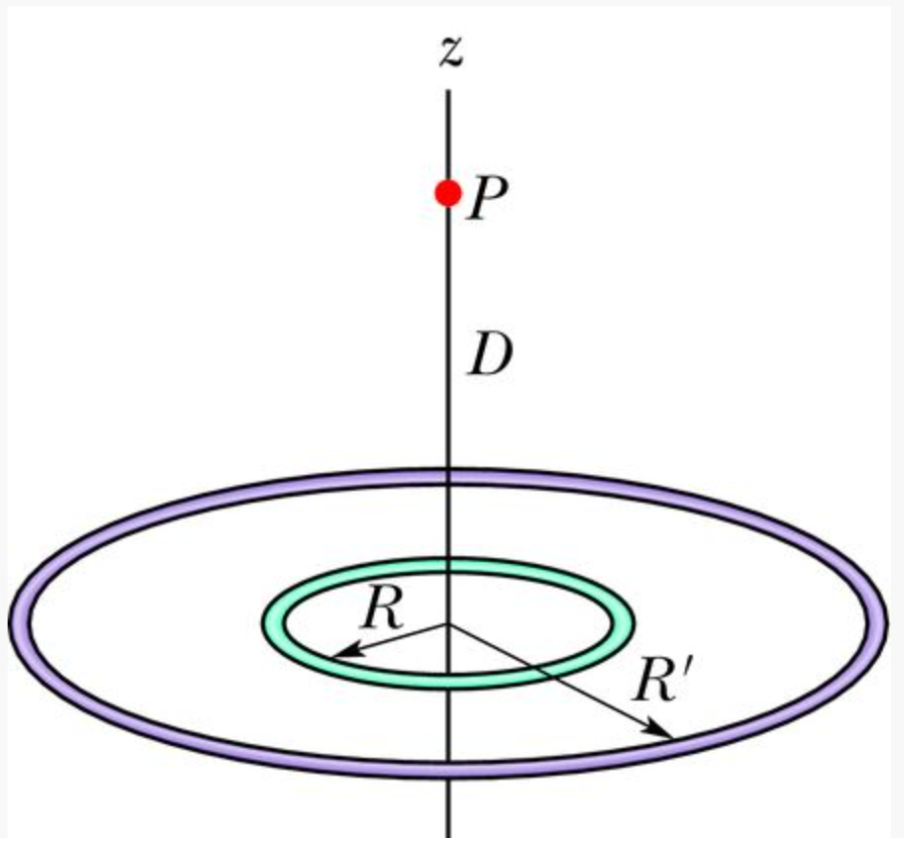
\includegraphics[width=0.25\textwidth]{picture_3.png} 
    % \label{fig:wrapfig}
\end{wrapfigure}
Figure 22-53 shows two concentric rings, of radii $R$ and $R' = 3.00R$, that lie on the same plane. Point $P$ lies on the central z axis, at distance $D = 2.00R$ from the center of the rings. The smaller ring has uniformly distributed charge $+Q$. In terms of $Q$, what is the uniformly distributed charge on the larger ring if the net electric field at $P$ is zero?

\subsection*{Solution: -13Q/5}
We begin with the fact that the net electric field is zero, and we expand on that.
We will call the charge on the outer ring $Q'$.
\begin{align*}
    E   &=  0
        =   E_R + E_{R'}
        =   \frac{kQ}{D^2 + R^2} + \frac{kQ'}{D^2 + R'^2}\\
        &=  \frac{kQ}{(2R)^2 + R^2} + \frac{kQ'}{(2R)^2 + (3R)^2}\\
        &=  \frac{kQ}{4R^2 + R^2} + \frac{kQ'}{4R^2 + 9R^2}
\end{align*}

From here, we can solve for $Q'$.
\begin{gather*}
    0   =   \frac{kQ}{5R^2} + \frac{kQ'}{13R^2}\\
    \frac{kQ}{5R^2}  =   -\frac{kQ'}{13R^2}\\
    \frac{Q}{5R^2}  =   -\frac{Q'}{13R^2}\\
    -\frac{Q}{5}  =   \frac{Q'}{13}\\
    Q'  =   \boxed{-\frac{13}{5}Q}
\end{gather*}
\pagebreak
\section{Chapter 23, Problem 42}
Two large metal plates of area $1.0 \unit{\meter^2}$ face each other, $5.0 \unit{\centi\meter}$ apart, with equal charge magnitudes $|q|$ but opposite signs. The field magnitude $E$ between them (neglect fringing) is $55 \unit{\newton/\coulomb}$. Find $|q|$.

\subsection*{Solution: 4.8675 \texttimes\ 10$^{-10}$ F}
We will treat the metal plates as a capacitor.
There exists a formula for the charge separated by a capacitor.
\[
    q   =   CV
\]

There are two variables in this that we need to find: the capacitance and the voltage.
\begin{gather*}
    C   =   \frac{\varepsilon_0 A}{d} = \frac{\varepsilon_0 * 1}{0.05} \unit{\farad}
        =   20\varepsilon_0\\
    \Delta V    =   -E \Delta x
        =   -55 * 0.05 \unit{\volt}
\end{gather*}

We can combine these into out above equation to get the answer.
\begin{gather*}
    q   =   CV
        =   (\frac{\varepsilon_0}{0.05}) * (-55 * 0.05)
        =   -55 * \varepsilon_0
        =   -4.8675 \times 10^{-10}\\
    |q| =   \boxed{4.8675 \times 10^{-10} \unit{\coulomb}}
\end{gather*}

\pagebreak
\section{Chapter 24, Problem 64}
A hollow metal sphere has a potential of +400 V with respect to ground (defined to be at V = 0) and a charge of $5.0 \times 10^{-9} \unit{\coulomb}$. Find the electric potential at the center of the sphere.

\subsection*{Solution: +400V}
The electric potential at the edge of the sphere is going to be $+400 \unit{\volt}$.
We know that the electric field inside a nonconducting sphere at any point is zero. 
Since the electric potential difference is the integral of the electric field, the change in electric potential is the area under the curve of the electric field.
Since the electric field is zero inside the shell at all points, the area under the curve would be just that: zero.
As such, we need but add the initial electric potential to this, leaving us with a final result of \boxed{+400 \unit{\volt}}

\pagebreak
\section{Chapter 24, Problem 67}
A metal sphere of radius 15 cm has a net charge of $3.0 \times 10^{-8} \unit{\coulomb}$. (a) What is the electric field at the sphere's surface? (b) If V = 0 at infinity, what is the electric potential at the sphere's surface? (c) At what distance from the sphere's surface has the electric potential decreased by 500 V?

\subsection{Solution: 11.987 \texttimes 10$^4$ N/C}
Let's use Gauss' Law for starters. 
\begin{gather*}
    \frac{q_{enc}}{\varepsilon_0} = \oint \vec{E} \cdot\,d\vec{A}\\
    \frac{q_{enc}}{\varepsilon_0} = E * 4\pi r^2\\
    E   =   \frac{kq_{enc}}{r^2}
        =   \frac{k*3.0 \times 10^{-8}}{0.15^2}
        =   \frac{(8.99 \times 10^9) * (3.0 \times 10^{-8})}{225 \times 10^{-4}}\\
    E   =   \frac{26.97 \times 10^{5}}{225}
        =   \boxed{11.987 \times 10^4 \unit{\newton/\coulomb}}
\end{gather*}

\subsection{Solution: 1789 V}
We prevoiusly established the formula for the electric field outside the shell.
\begin{equation*}
    E = \frac{kq_{enc}}{r^2}
\end{equation*}

We have a formula for the potential difference from the electric field.
\begin{align*}
    V   &=  -\int \vec{E}\cdot d\vec{s}
\end{align*}

Our limits would be from infinitely far away. 
Additionally, we would be travelling from there along the same line as the electric field, making $\cos(\theta) = 1$, so we can simplify the formula. 
\begin{align*}
    V   &=  -\int \frac{kq_{enc}}{r^2} \,dr
        =   -\left(-\frac{kq_{enc}}{r}\right) + c
        =   \frac{kq_{enc}}{r} + c
\end{align*}

Since $V = 0$ at infinity, and \(\lim_{r \to \inf}\left(\frac{kq_{enc}}{r}\right) = 0\), the constant c would be equal to the same (0).
This simplifies our equation immensely, and we can then just calculate the electric potential from the given information.
\begin{align*}
    V   &=  \frac{kq_{enc}}{r}
        =   \frac{(8.99 \times 10^9)*(3.0 \times 10^{-8})}{15 \times 10^{-1}}
        =   \frac{26.97 \times 10}{1.5 \times 10^{-1}}
        =   17.98 \times 10^2 
        =   \boxed{1798 \unit{\volt}}
\end{align*}

\subsection{Solution: 5.778cm}
When the electric potential has decreased by 500V, the electric potential will be $1798$V $-\ 500$V $= 1298$V. 
From this, we just have to find the value of $r$ where our formula applies.
\begin{align*}
    1298 \unit{\volt}   &=  \frac{kq_{enc}}{r}\\
    r   &=  \frac{(8.99 \times 10^9)*(3.0 \times 10^{-8})}{1298}\\
        &=  \frac{2697 \times 10}{1298}
        =   207.78 \times 10^{-3} \unit{\meter}\\
        &=  0.20778 \unit{\meter}
\end{align*}

This is the distance from the center for which the electric potential decreases by 500V.
Lastly, we just have to subtract the initial value.
\begin{equation*}
    0.20778 - 0.15 = \boxed{0.05778 \unit{\meter}}
\end{equation*}

\pagebreak
\section{Chapter 24, Problem 37}
What is the magnitude of the electric field at the point $(3.00\hat{i} - 2.00\hat{j} + 4.00\hat{k}) \unit{\meter}$ if the electric potential in the region is given by $V = 2.00xyz^2$, where V is in volts and coordinates $x$, $y$, and $z$ are in meters?

\subsection*{Solution: 125.0 N/C}
This problem is solvable using gradients and vectors.
\begin{align*}
    \vec{E} &=  \nabla V
        =   \left(\begin{smallmatrix} \diffp{V}{x}\\ \\ \diffp{V}{y}\\ \\ \diffp{V}{z} \end{smallmatrix}\right)
        =   \begin{pmatrix} 2yz^2\\ 2xz^2\\ 4xyz \end{pmatrix}\\
    \vec{E}(3, -2, 4)   &=  \begin{pmatrix} 2*(-2)*4^2\\ 2*3*4^2\\ 4*3*(-2)*4 \end{pmatrix}
        =   \begin{pmatrix} -64 \\ 96 \\ -48 \end{pmatrix} \unit{\meter}
\end{align*}

Knowing the vector value, we take the magnitude.
\begin{align*}
    \left|\vec{E}(3, -2, 4)\right|  &=  \sqrt{64^2 + 96^2 - 48^2}
        =   \sqrt{4096 + 9216 + 2304}\\
        &=  \sqrt{15616}
        =   \boxed{16 \sqrt{61} \unit{\newton/\coulomb} \approx 125.0 \unit{\newton/\coulomb}}
\end{align*}

\pagebreak
\section{Chapter 25, Problem 1}
\begin{wrapfigure}{r}{0.25\textwidth}
    \vspace{-30pt}
    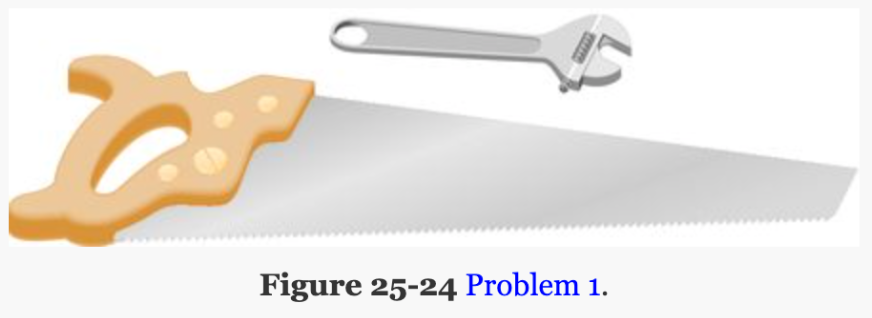
\includegraphics[width=0.25\textwidth]{picture_8.png} 
    % \label{fig:wrapfig}
\end{wrapfigure}
The two metal objects in Fig. 25-24 have net charges of $+70 \unit{\pico\coulomb}$ and $-70 \unit{\pico\coulomb}$, which result in a 20 V potential difference between them. (a) What is the capacitance of the system? (b) If the
charges are changed to $+200 \unit{\pico\coulomb}$ and $-200 \unit{\pico\coulomb}$, what does the capacitance become? (c) What does the potential difference become?

\subsection{Solution: 3.5 \texttimes\ 10$^{-12}$ F}
We have a friendly equation involving capacitance that we can use.
\begin{align*}
    q   &=  CV\\
    C   &=  \frac{q}{V}
        =   \frac{70 \times 10^{-12} \unit{\coulomb}}{20 \unit{\volt}}
        =   \boxed{3.5 \times 10^{-12} \unit{\farad}}
\end{align*}

\subsection{Solution: 3.5 \texttimes\ 10$^{-12}$ F}
While capactance is calculatable from the charge, it is not dependant on it. 
Thus, the capacitance stays the same at \boxed{3.5 \times 10^{-12} \unit{\farad}}.

\subsection{Solution: 57.143 V}
In order for the above equation ($q = CV$) to remain accurate, the potential difference must increase by the same multiplicative factor.
From 70 to 200, there is a multiplication factor of $\frac{20}{7}$. 
We should multiply the electrical potential difference by that same factor.
\begin{equation*}
    20 \unit{\volt} * \frac{20}{7} = \boxed{\frac{400}{7} \unit{\volt} \approx 57.143 \unit{\volt}}
\end{equation*}

\end{document}